\input{preamble.tex}
\usepackage{makecell} % commande \thead, dans l'exo 1
\usepackage{eurosym} % pour le symbole euro propre

\begin{document}

\reversemarginpar

\pagestyle{fancy}
\fancyhead[L]{Terminale STMG}
\fancyhead[C]{\textbf{DS n°4 - Fonction inverse et polynômes - 1a}}
\fancyhead[R]{\today}

\null\vspace{-30pt}
Nom / Prénom : \\

Consignes particulières : 
\begin{itemize}[label=$\bullet$]
	\item 
	La calculatrice est {autorisée}.
	\item 
	L'exercice \ref{exe:1a} peut être fait entièrement sur la feuille d'évaluation. Écrire son nom avant de rendre le sujet pour qu'il soit corrigé.
	\item 
	Toute trace de recherche est prise en compte.
%	\item 
%	L'abbréviation $\tq$ signifie ``tel que''.
\end{itemize}

\hrule

\exe{4}{
Compléter les phrases ci-dessous :
\begin{enumerate}
\item
La dérivée du polynôme $x \mapsto ax^3 + cx + d$ est $\dots$
\item
La dérivée de la fonction $x \mapsto \dfrac{a}{x}$ sur $\Ret$ est $\dots$
\item 
Le polynôme $8x - 3x^2 + 7$ est de degré $\dots$
\item
La fonction $x \mapsto \dfrac{1}{x}$ est appelée $\dots$
\end{enumerate}
}{exe:1a}{
\begin{enumerate}
\item
La dérivée du polynôme $x \mapsto ax^3 + cx + d$ est $x \mapsto 3ax^2 + c$.
\item
La dérivée de la fonction $x \mapsto \dfrac{a}{x}$ sur $\Ret$ est $x \mapsto - \dfrac{a}{x^2}$.
\item 
Le polynôme $8x - 3x^2 + 7$ est de degré 2.
\item
La fonction $x \mapsto \dfrac{1}{x}$ est appelée fonction inverse.
\end{enumerate}
}

\exe{4}{
Donner les fonctions dérivées des fonctions suivantes sur $\Ret$ :
\begin{multicols}{2}
\begin{enumerate}
\item $f: x \mapsto 4x^2 - \frac5{x} + 3x$
\item $f: x \mapsto -12x^3  +\frac57 x^2 - 4 + \frac8{x}$
\item $f: x \mapsto x - x + x + \frac7{3x}$
\item$f: x \mapsto x^3 - \frac{3}2x^2 + 3x -3 - \frac{12}{x}$
\end{enumerate}
\end{multicols}
}{exe:2a}{
\begin{multicols}{2}
\begin{enumerate}
\item $f: x \mapsto 8x + \frac5{x^2} + 3$
\item $f: x \mapsto -36x^2  +\frac{10}7 x - \frac8{x^2}$
\item $f: x \mapsto 1 - \frac7{3x^2}$
\item$f: x \mapsto 3x^2 - 3x + 3 + \frac{12}{x^2}$
\end{enumerate}
\end{multicols}
}

\exe{4}{
Etudier les variations des fonctions suivantes sur $\R$. Si possible, donner le maximum ou le minimum de la fonction.
\begin{enumerate}
\item $f: x \mapsto -3x^2 +18x + 32$
\item $f: x \mapsto \frac{15}2 x^2 + 5 x - 2$
\end{enumerate}
}{exe:3a}{
\begin{enumerate}
\item La dérivée est $f'(x) = -6x +18$ qui s'annule en $x=3$. Le tableau de variation est donné ci-dessous :
\begin{center}
\begin{tikzpicture}
   \tkzTabInit{$x$ / 1 , $f'(x)$ / 1, $f(x)$ / 1.5}{$-\infty$, $3$, $\infty$}
   \tkzTabLine{, +, z, -, }
   \tkzTabVar{ -/ , +/ $59$ , -/ }
\end{tikzpicture}
\end{center}
Le maximum est $f(3) = 59$.
\item La dérivée est $f'(x) = 15x +5$ qui s'annule en $x=-\frac13$. Le tableau de variation est donné ci-dessous :
\begin{center}
\begin{tikzpicture}
   \tkzTabInit{$x$ / 1 , $f'(x)$ / 1, $f(x)$ / 1.5}{$-\infty$, $-\frac13$, $\infty$}
   \tkzTabLine{, -, z, +, }
   \tkzTabVar{ +/ , -/ $-\frac{17}6$ , +/ }
\end{tikzpicture}
\end{center}
Le minimum est $f \bigpar{-\frac13} = -\frac{17}6$.
\end{enumerate}
}

\exe{8}{
Etudier les variations des fonctions suivantes sur $\Ret$ :
\begin{multicols}{2}
\begin{enumerate}
\item $f: x \mapsto 4x - 8 + \frac{12}x$
\item $f: x \mapsto 2x - 426 + \frac{242}{x}$
\item $f: x \mapsto-2x + 7 + \frac{5}{x}$
\item $f: x \mapsto-4x + 31 - \frac{144}{x}$
\end{enumerate}
\end{multicols}
}{exe:4a}{
\begin{enumerate}

\item La dérivée est $f'(x) = 4 - \frac{12}{x^2}$ qui s'annule en $-\sqrt{3}$ et en $\sqrt{3}$.
Le tableau de variation est donné ci-dessous :
\begin{center}
\begin{tikzpicture}
   \tkzTabInit{$x$ / 1 , $f'(x)$ / 1, $f(x)$ / 1.5}{$-\infty$, $-\sqrt{3}$, $0$, $\sqrt{3}$, $+\infty$}
   \tkzTabLine{, +, z, -, d, -, z, +, }
   \tkzTabVar{-/ , +/, -DC+/, -/, +/ }
\end{tikzpicture}
\end{center}

\item La dérivée est $f'(x) = 2 - \frac{242}{x^2}$ qui s'annule en $-11$ et en $11$.
Le tableau de variation est donné ci-dessous :
\begin{center}
\begin{tikzpicture}
   \tkzTabInit{$x$ / 1 , $f'(x)$ / 1, $f(x)$ / 1.5}{$-\infty$, $-11$, $0$, $11$, $+\infty$}
   \tkzTabLine{, +, z, -, d, -, z, +, }
   \tkzTabVar{-/ , +/, -DC+/, -/, +/ }
\end{tikzpicture}
\end{center}

\item La dérivée est $f'(x) = -2 - \frac{5}{x^2}$ qui est toujours négative.
Le tableau de variation est donné ci-dessous :
\begin{center}
\begin{tikzpicture}
   \tkzTabInit{$x$ / 1 , $f'(x)$ / 1, $f(x)$ / 1.5}{$-\infty$, $0$, $+\infty$}
   \tkzTabLine{, -, d, -, }
   \tkzTabVar{+/ , -DC+/, -/ }
\end{tikzpicture}
\end{center}

\item La dérivée est $f'(x) = -4 + \frac{144}{x^2}$ qui s'annule en $-6$ et $6$.
Le tableau de variation est donné ci-dessous :
\begin{center}
\begin{tikzpicture}
   \tkzTabInit{$x$ / 1 , $f'(x)$ / 1, $f(x)$ / 1.5}{$-\infty$, $-6$, $0$, $6$, $+\infty$}
   \tkzTabLine{, -, z, +, d, +, z, -, }
   \tkzTabVar{+/ , -/, +DC-/, +/, -/ }
\end{tikzpicture}
\end{center}

\end{enumerate}
}

%%%%%%%%%%%%

\setcounter{Exercise}{0}

\newpage

\pagestyle{fancy}
\fancyhead[L]{Terminale STMG}
\fancyhead[C]{\textbf{DS n°4 - Fonction inverse et polynômes - 1b}}
\fancyhead[R]{\today}

\null\vspace{-30pt}
Nom / Prénom : \\

Consignes particulières : 
\begin{itemize}[label=$\bullet$]
	\item 
	La calculatrice est {autorisée}.
	\item 
	L'exercice \ref{exe:1b} peut être fait entièrement sur la feuille d'évaluation. Écrire son nom avant de rendre le sujet pour qu'il soit corrigé.
	\item 
	Toute trace de recherche est prise en compte.
%	\item 
%	L'abbréviation $\tq$ signifie ``tel que''.
\end{itemize}

\hrule

\exe{4}{
Compléter les phrases ci-dessous :
\begin{enumerate}
\item
La fonction $x \mapsto \dfrac{1}{x}$ est appelée $\dots$
\item 
Le polynôme $8x - 3x^3 + 7$ est de degré $\dots$
\item
La dérivée du polynôme $x \mapsto ax^3 + bx^2 + d$ est $\dots$ 
\item
La dérivée de la fonction $x \mapsto - \dfrac{a}{x}$ sur $\Ret$ est $\dots$
\end{enumerate}
}{exe:1b}{
\begin{enumerate}
\item
La fonction $x \mapsto \dfrac{1}{x}$ est appelée fonction inverse.
\item 
Le polynôme $8x - 3x^3 + 7$ est de degré 3.
\item
La dérivée du polynôme $x \mapsto ax^3 + bx^2 + d$ est $x \mapsto 3ax^2 + 2bx$.
\item
La dérivée de la fonction $x \mapsto - \dfrac{a}{x}$ sur $\Ret$ est $x \mapsto + \dfrac{a}{x^2}$ \\
\end{enumerate}
}

\exe{4}{
Donner les fonctions dérivées des fonctions suivantes sur $\Ret$ :
\begin{multicols}{2}
\begin{enumerate}
\item $f: x \mapsto x - x + x + \frac3{7x}$
\item $f: x \mapsto 9x^3  - \frac37 x^2 - 4 + \frac8{x}$
\item$f: x \mapsto x^3 + \frac{5}2x^2 - 7x -3 + \frac{12}{x}$
\item $f: x \mapsto 7x^2 + 3x + \frac5{x}$
\end{enumerate}
\end{multicols}
}{exe:2b}{
\begin{multicols}{2}
\begin{enumerate}
\item $f: x \mapsto 1 - \frac3{7x^2}$
\item $f: x \mapsto 27x^2  +\frac{6}7 x - \frac8{x^2}$
\item$f: x \mapsto 3x^2 - 5x^2 - 7 + 3 - \frac{12}{x^2}$
\item $f: x \mapsto 14x + 3 - \frac5{x^2}$
\end{enumerate}
\end{multicols}
}

\exe{4}{
Etudier les variations des fonctions suivantes sur $\R$. Si possible, donner le maximum ou le minimum de la fonction.
\begin{multicols}{2}
\begin{enumerate}
\item $f: x \mapsto -\frac{15}2 x^2 - 5 x + 2$
\item $f: x \mapsto 3x^2 -18x - 32$
\end{enumerate}
\end{multicols}
}{exe:3b}{
\begin{enumerate}

\item La dérivée est $f'(x) = -15x -5$ qui s'annule en $x=-\frac13$. Le tableau de variation est donné ci-dessous :
\begin{center}
\begin{tikzpicture}
   \tkzTabInit{$x$ / 1 , $f'(x)$ / 1, $f(x)$ / 1.5}{$-\infty$, $-\frac13$, $\infty$}
   \tkzTabLine{, +, z, -, }
   \tkzTabVar{ -/ , +/ $\frac{17}6$ , -/ }
\end{tikzpicture}
\end{center}
Le maximum est $f \bigpar{-\frac13} = \frac{17}6$.

\item La dérivée est $f'(x) = 6x -18$ qui s'annule en $x=3$. Le tableau de variation est donné ci-dessous :
\begin{center}
\begin{tikzpicture}
   \tkzTabInit{$x$ / 1 , $f'(x)$ / 1, $f(x)$ / 1.5}{$-\infty$, $3$, $\infty$}
   \tkzTabLine{, -, z, +, }
   \tkzTabVar{ +/ , -/ $-59$ , +/ }
\end{tikzpicture}
\end{center}
Le minimum est $f(3) = -59$.

\end{enumerate}
}

\exe{8}{
Etudier les variations des fonctions suivantes sur $\Ret$ :
\begin{multicols}{2}
\begin{enumerate}
\item $f: x \mapsto 2x + 7 - \frac{5}{x}$
\item $f: x \mapsto -4x + 8 + \frac{12}x$
\item $f: x \mapsto -2x - 426 - \frac{242}{x}$
\item $f: x \mapsto 4x + 31 + \frac{144}{x}$
\end{enumerate}
\end{multicols}
}{exe:4b}{
\begin{enumerate}
\item La dérivée est $f'(x) = 2 + \frac{5}{x^2}$ qui est toujours positive.
Le tableau de variation est donné ci-dessous :
\begin{center}
\begin{tikzpicture}
   \tkzTabInit{$x$ / 1 , $f'(x)$ / 1, $f(x)$ / 1.5}{$-\infty$, $0$, $+\infty$}
   \tkzTabLine{, +, d, +, }
   \tkzTabVar{-/ , +DC-/, +/ }
\end{tikzpicture}
\end{center}

\item La dérivée est $f'(x) = -4 - \frac{12}{x^2}$ qui est toujours négative.
Le tableau de variation est donné ci-dessous :
\begin{center}
\begin{tikzpicture}
   \tkzTabInit{$x$ / 1 , $f'(x)$ / 1, $f(x)$ / 1.5}{$-\infty$, $0$, $+\infty$}
   \tkzTabLine{, -, d, -, }
   \tkzTabVar{+/ , -DC+/, -/ }
\end{tikzpicture}
\end{center}

\item La dérivée est $f'(x) = -2 + \frac{242}{x^2}$ qui s'annule en $-11$ et en $11$.
Le tableau de variation est donné ci-dessous :
\begin{center}
\begin{tikzpicture}
   \tkzTabInit{$x$ / 1 , $f'(x)$ / 1, $f(x)$ / 1.5}{$-\infty$, $-11$, $0$, $11$, $+\infty$}
   \tkzTabLine{, -, z, +, d, +, z, -, }
   \tkzTabVar{+/ , -/, +DC-/, +/, -/ }
\end{tikzpicture}
\end{center}

\item La dérivée est $f'(x) = 4 - \frac{144}{x^2}$ qui s'annule en $-6$ et $6$.
Le tableau de variation est donné ci-dessous :
\begin{center}
\begin{tikzpicture}
   \tkzTabInit{$x$ / 1 , $f'(x)$ / 1, $f(x)$ / 1.5}{$-\infty$, $-6$, $0$, $6$, $+\infty$}
   \tkzTabLine{, +, z, -, d, -, z, +, }
   \tkzTabVar{-/ , +/, -DC+/, -/, +/ }
\end{tikzpicture}
\end{center}

\end{enumerate}

}

%%%%%%%%%%%%

\newpage
\fancyhead[C]{\textbf{Solutions}}
Les solutions sont données dans l'ordre sujet a puis b. \newline
\shipoutAnswer


\end{document}
